\chapter{序論}
%章番号が不要な場合は『\chapter*{概要}』とする
\section{はじめに}%-----------No.1--------------------------------------
\subsection{ロボットの社会実装}
近年,安全安心で持続可能な社会の実現,少子高齢化対応や第一次産業を始めとした産業基盤の構築等の社会的な課題に対する解決策として,ロボットの社会実装が期待されている.\\
ここで,ロボットの社会実装の社会的期待について考えるため,工場内でのロボット有用を例にとる.産業用ロボットの普及に伴い,工場内でのロボット実装には労働者を守るための安全対策が複数関わってくる.代表的なものとして,労働安全規則や国際標準化機構(International Organization for Standardization: ISO), 日本工業規格(Japanese Industrial Standards: JIS)などが挙げられる.労働安全衛生規則第150条の4では,\\
 \underline{事業者は、産業用ロボットを運転する場合(教示等のために産業用ロボットを運転する場合及}\\
 \underline{び産業用ロボットの運転中に次条に規定する作業を行を行わなければならない場合において}\\
 \underline{産業用ロボットを運転するときを除く。)において、当該産業用ロボットに接触することに}\\
 \underline{より労働者に危険が生ずる恐れのあるときは、さく又は囲いを設ける等当該危険を防止する}\\
 \underline{ために必要な措置を講じなければならない。)}\\
  とある.この規則により,人間とロボとslack が同じ工場内で作業する場合において,その間には,柵や囲いを設ける必要があり,協働することは困難であった.しかし,規制改革実施計画及び近年の技術改心が加味され,平成25年12月24日付基発1224第2号通達によりいかが明記された.\\
 \underline{産業用ロボットを使用する事業者が,労働安全衛生第28条の2による危険性等の調査(以下}\\
 \underline{「リスクアセスメント」という。)に基づく措置を実施し、産業用ロボットに接触することに}\\
 \underline{より労働者の危険の生ずるおそれが無くなったと評価できるときは、本条の「労働者に危険が}\\
 \underline{生ずるおそれがあるとき」に{\bf 該当しない}ものとすること。}(以下省略)\\
したがって,現在では安全が確保できていると確認できる環境下であれば,人間とロボットが協働作業可能となった.\\
このように,法整備という観点から観察しても,社会的期待としては人間とロボットが同じフィールドで安心して作業や生活さえも行える将来が望まれている.しかし,度ボットにかんする研究開発では,「人とロボットの関係性」についてどこまで考えられているであろうか.ロボットの社会実装には,社会的期待と研究開発との方向性の乖離を避け,研究成果をわかりやすく社会に還元・提示する必要がある.そのため,人間とロボットをどのように共存させるか,人間ロボット共生社会のあり方を議論すべきである.
\subsection{協調行動}
協調行動は, 異なる自律エージェントが共通のタスクを実行しながらコミュニケーションを図るときに重要な側面である. 多くの場合,単一のエージェントでのタスクを実行は必ずしも効率的とは言えず, ここ数年で, 困難な問題を解決するためにマルチエージェントシステム(MAS)を研究している研究者も多い. マルチエージェントシステムは, 複数のエージェント(自律エージェント)が協調行動によって共通の目標を達成しようとするシステムである .  センサーから取得したデータに基づいてリアルタイムで決定を下すことによって, エージェント同士に加え,環境と相互作用する. %\cite{PS}\cite{KU}
MASのテストベッドとして有名な,RoboCupは,世界的ロボット大会であり,強化学習やニューラルネットワークなどの学習方法を使用してマルチエージェントの協調を一つの課題としている.  RoboCupはランドマークプロジェクトであり,2050年までに,人間のサッカーワールドカップチャンピオンチームに勝つロボットチームの制作プロジェクトである%\cite{BS}. 
例としてこれまでに,Sandholm and Crites[??]によれば, 十分な測定データと行動が利用可能であれば, 強化学習は反復囚人のジレンマに対して最適な手法であると示された. さらに, Arai[??]は, 環境がグリッドとしてモデル化されている場合のマルチエージェントシステムにおける追跡問題に関するQラーニングと利益共有の方法を比較し, 協力的な行動が利益共有の間で明確に現れることを示した. しかしながら, これらの研究は, 実環境で動作するロボットへの応用をまだ考慮されていない. 

\subsection{ロボット学習}
学習アルゴリズムの中で,教師なし学習はMASシステムにとって有望な方法である.教師なし学習の利点は,ロボットが環境に関する以前の情報やロボット自体の前提知識を持っている必要がないことである. しかし,学習には多くのテストや経験が必要であるため, 設計者は, 状態空間とアクション空間を定義するために, 試合中に考慮すべき重要なパラメータと変数を明確に定義することがコストと時間を削減するために重要である. 状態空間の設計は, ロボットが行動空間で何ができるかによって異なる. 同時に, 状態空間はロボットの能力とそれ自身の行動空間に従って定義される. 2つの空間は互いに相互接続している. 効率的な方法で状態空間を設計するために, Asada[??]は, 状態空間を最初に2つの主な状態に分割し, 次に状態数を増やしながら再帰的に多数の層に分割する方法を提案した. しかし, いくらかの偏りの問題は依然としてロボットの行動に影響を及ぼし, 何らかの誤った行動および習慣を引き起こす可能性があると示された.

\subsection{人間ロボット協調}
前節で述べたように,複数の実ロボット間での協調行動の獲得においては,様々な議論がなされてきた.しかし,人間ロボット共生社会を見据えた際に,これまでの学習に対する観察対象がロボットであることに,疑問を呈する.事実,インタフェースの問題を度外視しても,人間と現在のマルチエージェントシステムを用いたロボット群との意思伝達は容易ではない.そこで,本研究では,人間同士による協調行動を観察しロボットに応用することを考える.(Fig. \ref{fig:01_01}参照) 実ロボットの学習において,課題として挙げられていた,経験の偏りや、環境認識における状態空間からの入力ベクトル要素の選定について,ニューラルネットワークを用いて,検討する.本稿では,まずSOMを用いて人間の協調行動におけるポジションによる状況分析を行う.人間の協調行動の観察対象として,今回はフットサルの試合を用いる.複数のエージェントの協調によって目的が達成され,環境が動的に変化し,多目的・多重制約問題を全て包括し,かつ実時間計画・推論を必要とする点において,人間ロボット共生社会での課題と一致するからである.
 また,人間同士による協調行動を評価するために,ロボット同士による協調行動についても,観察を行う.観察対象は,ロボカップサッカーにおける中型リーグの試合である.ロボカップについては次章に記す.\\
ニューラルネットワークへの入力ベクトルの要素は,人間とロボットの行動との間の可能な最小のギャップを達成するように選択される.そのためには, まず人間の行動を理解し,そのような行動を理解して模倣できるロボットを開発することが重要でである.文献[??]では,フットサルゲームにおける人間とロボットの行動の研究に焦点を当てている.なぜなら,これは動的な環境,いくつかの制約を伴う優れたテストベッドであり,リアルタイムの計画が必要だからである.これらは,ロボットが将来動作する可能性がある一般的な共生システムの特性となる.使用されるアルゴリズムでは,スコア,コーナーキック,ペナルティキック,ボールを持っているチームなど,ゲーム内の特定のイベントに応じて,SOMを使用してプレーヤーのポジションが分析された. その結果,人間の試合もロボットの試合も同様に, 試合における場面を評価することが可能であり, 学習する入力要素を増やすことによって,環境と行動の写像関係を示すSOMの作成によってロボットによる自律的行動の発現が可能であることが判明した. この論文では,その写像関係を求め,テンソル自己組織化マップによりロボット同士の試合を学習し,サッカーロボットの行動学習システムの開発を行う.

\subsection{ロボカップ}%-----------
ロボカップとは「2050年までに人間のW杯優勝チームにかつ自律ロボットチームを作る」という大きな目標を掲げた国際ランドマークプロジェクトである.サッカーというテーマは,動的な環境下で囚人に判断をする知能や,マクドナルド システムによるチーム行動といった要素を有している.しかし,サッカーというテーマだけでなく,ロボカップでは,人間のせい買う空間であるキッチンやリビングを再現したフィールドで競技を行う「@ホームリーグ」や,災害現場で教授に役立つ自律ロボット開発を推進する「レスキューリーグ」,次世代の人材育成を目的とした「ジュニアリーグ」,2012年から追加された「インダスリアルリーグ」など,「サッカーリーグ」を含めて現在では5つのリーグが存在し,様々な分野の技術を発展させるプロジェクトとなっている.各リーグで共通する課題は,「複数ロボットの協調によって目的は達成され,かんきょうが動的に変化し,多目的/多重制約問題を包含し,実時間計画/推論を必要とすること」である.\\
筆者が所属するチーム「Hibikino-Musashi」は,サッカーリーグの中の,「ロボカップサッカー中型ロボットリーグ(Middle Size League)」(Fig.~)である.

\subsubsection{ロボカップサッカー中型ロボットリーグ(MSL)}
中型ロボットリーグ(以下,MSLと表記する)では,年々フィールドのサイズが大きうくなっているが,現状では12[m]×18[m]の大きさのフィールドで試合を行うリーグである.各チームの試合に参加可能なロボットは5台までとなっており,ロボットの大きさは52[cm]×52[cm],高さ80[cm]以下となっている.(ゴールキーパーロボットは1秒間のみ,60[cm]×60[cm],高さ90[cm]まで拡大可能)ロボットは搭載されたカメラなどのセンサ情報から環境認識し,自律行動を行う.試合は前後半15分の合計30分間行われる.

\subsubsection{試合データ}
ロボカップサッカー中型リーグでは,2017年から試合中のロボットの自己位置・障害物認識状態などの情報をリアルタイムに近い状態で,提出することが義務かされるようになった.これは,試合中のデバッグ用だけでなく統計分析のためのデータ標準化でのある.\\
提出された全参加チームデータは,インターネット情に公開され,研究・開発その他に誰でも利用可能である.ロボットや障害物,ボールに関する全ての座標データは,どのチームも定義された3次元空間のデカルト座標系で提出しなければならない.

\clearpage

\begin{figure}[ht]
  \begin{center}
  
    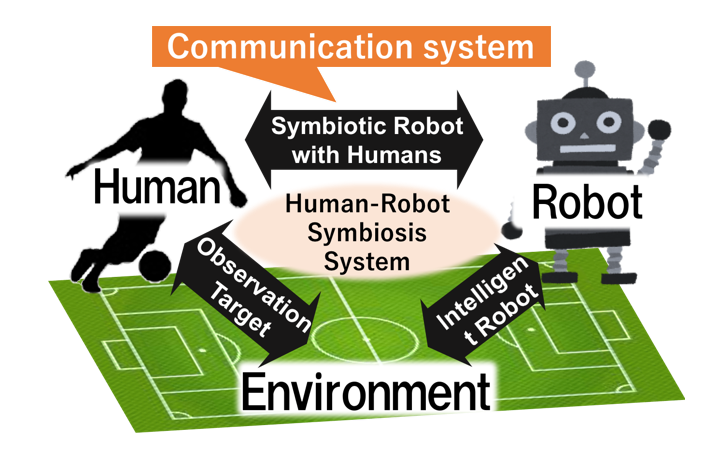
\includegraphics[clip,width=15.0cm]{figure/01_01_Human-Robot_Symbiosis_System.eps}
    \caption{Human-Robot Symbiosis System}
    \label{fig:01_01}
    
    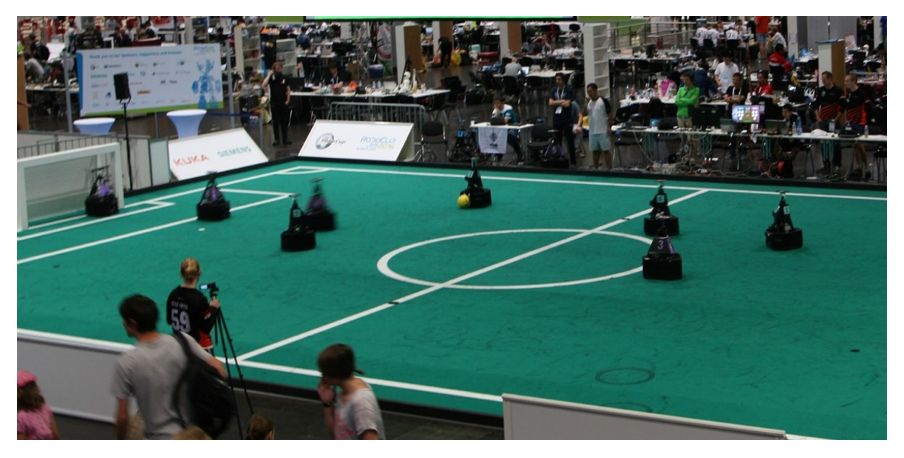
\includegraphics[width=15.0cm]{figure/01_02_RoboCup_Middle_Size_League_2016.eps}
    \caption{RoboCup Middle Size League 2016}
    \label{fig:01_02}
    
  \end{center}
\end{figure}

\clearpage
%-----------No.1--------------------------------------


\section{本研究の目的}%-----------No.2--------------------------------------
本研究の目的は,人間のチームとしての行動決定アルゴリズムを解析し,教師なし学習である自己組織化マップを用いて,近似されたモデルを用い,ロボットに環境人氏から行動決定の写像関係を学習させることを目的とする.
%-----------No.2--------------------------------------


\section{本論文の構成}%-----------No.3--------------------------------------
本論文の構成は,第2章では,本研究において使用する自己組織化マップについての歴史とアルゴリズムを述べた上で人間のチーム行動の解析を行う.第3章では,第4章では,最後に第5章では,考察及びまとめを述べる.
%-----------No.3--------------------------------------



  \footnote{
%--------
補足があればここに...
} %--------











